% This work is licensed under the Creative Commons
% Attribution-NonCommercial-ShareAlike 4.0 International License. To view a copy
% of this license, visit http://creativecommons.org/licenses/by-nc-sa/4.0/ or
% send a letter to Creative Commons, PO Box 1866, Mountain View, CA 94042, USA.

\chapter{Brownsche Bewegung} %10

\begin{defi}\ %nonumber
	\begin{itemize}
		\item Ein stochastischer Prozess in \textbf{stetiger Zeit} ist eine messbare Abbildung 
\begin{align*}
	X\colon[0,T]\times\Omega\to\R^d,\qquad(t,\omega)\mapsto X_t(\omega).
\end{align*}
		\item Wir nennen $X$ einen \textbf{stetigen stochastischen Prozess}, wenn alle Pfade bis auf Nullmengen stetig sind, d.h.
		\begin{align*}
		:\Longleftrightarrow t\mapsto X_t(\omega)\text{ ist stetig }\qquad\forall \omega\in\Omega\setminus A \mit A~\P\text{-Nullmenge}
		\end{align*}
	\end{itemize}
\end{defi}

Die \textit{Brownsche Bewegung} ist:
\begin{itemize}
	\item stetige Verallgemeinerung von Random Walks
	\item Klassisches Modell für "zufällige Bewegung" in $\R^d$.
	\item Zur Ideengeschichte: 
	\begin{itemize}
		\item Zitterbewegung von Blütenpollen auf Wasser (Robert Brown 1828)
		\item \textit{Brownsche Molekularbewegung} (Einstein, Smolochowski 1909)
		\item Finanzmathematik: Zufällige Preisbewegungen (Bachelier 1900)
		\item Norbert Wiener (1923): erste rigorose mathematische Beschreibung\\
		Deshalb heißt die Brownsche Bewegung oft auch \textbf{Wiener Prozess}.
	\end{itemize}		
\end{itemize}

\begin{defi}
	Ein reellwertiger stochastischer Prozess $B:=(B_t)_{t\in[0,T]}$ heißt\\ \textbf{(standardisierte) Brownsche Bewegung (BB)}, wenn:
	\begin{enumerate}[label=\alph*)]
		\item $\begin{aligned}
			B_0=0
		\end{aligned}$ (Standardisierung)
		\item $B$ hat \textbf{unabhängige Zuwächse}, d.h. für beliebige Zeitpunkte\\ $0\leq t_1<t_2<\ldots<t_N\leq T$ sind die Zufallsvariablen
		\begin{align*}
			\left(B_{t_1}-B_0\right),\left(B_{t_2}-B_{t_1}\right),\ldots,\left(B_{t_N}-B_{t_{N-1}}\right)
		\end{align*}
		unabhängig.
		\item $\begin{aligned}
			\big(B_t-B_s\big)\sim\Nor(0,t-s)\qquad\forall 0\leq s\leq t\leq T
		\end{aligned}$  (\textbf{stationäre, normalverteilte Zuwächse})
		\item $B$ ist ein stetiger stochastischer Prozess.
	\end{enumerate}
\end{defi}

Alternative Charakterisierung als Gaußscher Prozess:

\begin{defi}
	Ein stochastischer Prozess $(X_t)_{t\in[0,T]}$ heißt \textbf{Gaußscher Prozess}
	\begin{align*}
		:\Longleftrightarrow \Big(X_{t_1},X_{t_2},\ldots,X_{t_N}\Big)\text{ (multivariat) normalverteilt ist }\forall0\leq t_1\leq t_2\leq\ldots\leq t_n\leq T  
	\end{align*}
	Hierbei sind $\big(X_{t_1},X_{t_2},\ldots,X_{t_N}\big)$ die \textbf{endlich-dimensionalen Randverteilungen}.
\end{defi}

\begin{lemma}\label{10.1}
	Sei $(X_t)_{t\in [0,T]}$ ein stetiger Gaußscher Prozess mit 
	\begin{itemize}
		\item $\begin{aligned}
			X_0=0
		\end{aligned}$
		\item $\begin{aligned}
			\E\big[X_t]=0 \hspace{90pt}\forall t\in[0,T]
		\end{aligned}$
		\item $\begin{aligned}
			\Cov\big(X_t,X_s\big)=\min(s,t) \qquad\forall s,t\in[0,T]
		\end{aligned}$
	\end{itemize}
	Dann ist $X$ eine Brownsche Bewegung.
\end{lemma}

\begin{proof}
	Zu zeigen: unabhängige Zuwächse und $\Var\big(X_t-X_s\big)=t-s$.\\
	Sei $X$ Gaußscher Prozess. 
	Setze $Y:=\big(X_{t_1},\ldots,X_{t_N}\big)\sim$ multivariat Normalverteilt.
	\begin{align*}
		\left(X_{t_2}-X_{t_1},\ldots,X_{t_N}-X_{t_{N-1}}\right)
		&=\begin{pmatrix}
			-1 & 1 & 0 & 0 & \hdots & 0\\
			0 & -1 & 1 & 0 & \hdots & \vdots\\
			0 & 0 & -1 & 1 & \hdots & \vdots\\
			\vdots & \ddots & \ddots & \ddots & \vdots & 0\\
			0 & \hdots & \hdots & 0 & -1 & 1
		\end{pmatrix}\cdot Y
	\end{align*}
	ist wieder multivariat normalverteilt.\\
	D.h. die Zuwächse sind unkorreliert!
	Sei $i\leq j$.
	\begin{align*}
		&\Cov\left(X_{t_j}-X_{t_{j-1}},X_{t_i}-X_{t_{i-1}}\right)\\
		&=\E\left[\left(X_{t_j}-X_{t_{j-1}}\right)\cdot\left(X_{t_i}-X_{t_{i-1}}\right)\right]\\
		&=\E\big[X_{t_j}\cdot X_{t_i}\big]-\E\big[X_{t_{j-1}}\cdot X_{t_i}\big]-\E\big[X_{t_j}\cdot X_{t_{i-1}}\big]+\E\big[X_{t_{j-1}}\cdot X_{t_{i-1}}\big]\\
		&=\min\lbrace t_j,t_i\rbrace-\min\lbrace t_{j-1},t_i\rbrace-\min\lbrace t_j,t_{i-1}\rbrace+\min\lbrace t_{j-1},t_{i-1}\rbrace\\
		&=t_i-t_i+t_{i-1}+t_{i-1}\\
		&=0
	\end{align*}
	
	Also sind die Zuwächse von $X$ unabhängig.
	Zur Varianz:
	\begin{align*}
		\Var\big(X_t-X_s\big)
		&=\E\left[\big(X_t-X-s\big)^2\right]\\
		&=\E\left[X_t^2-2\cdot X_s\cdot (X_t-X_s)-X_s^2\right]\\
		&=\underbrace{\E\big[X_t^2\big]}_{=t}-2\cdot\E\Big[\underbrace{\big(X_s-X_0\big)\cdot\big(X_t-X_s\big)}_{\unab}\Big]-\underbrace{\E\big[X_s^2\big]}_{=s}\\
		&=t-s
	\end{align*}
\end{proof}

\subsection*{\textbf{Wavelet-Konstruktion} der BB auf $[0,1]$:}
Betrachte den Hilbertraum $L_2([0,1])$ mit ONB $(\psi_k)_{k\in\N}$. (Später Haar-Wavelets)
\begin{align*}
	&\text{Inneres Produkt:} &\langle f,g\rangle&=\int\limits_0^1 f(x)\cdot g(x)\d x\\
	&\text{Parselvalsche Ungleichung:} &\langle f,g\rangle&=\sum\limits_{k=0}^\infty\langle f,\psi_k\rangle\cdot\langle g,\psi_k\rangle
\end{align*}
Seien $(Z_k)_{k\in\N}$ iid Folge von standardnormalverteilten Zufallsvariablen. Setze
\begin{align}\label{eqWaveletKonstruktionStern}\tag{$\ast$}
	B_t:=\sum\limits_{k=0}^\infty Z_k\cdot\int\limits_0^t\psi_k(s)\d s\qquad\forall t\in[0,1]
\end{align}
Behauptung: $B$ ist Brownsche Bewegung.\nl
Zu zeigen:
\begin{enumerate}[label=\alph*)]
	\item Summe konvergiert in $L_2([0,1])=L_2(\d\P)$ für jedes $t\in[0,1]$.
	\item $B$ ist gaußscher Prozess
	\item $\begin{aligned}
		\E\big[B_t\big]=0\text{ und }\Cov\big(B_t-B_s\big)=\min\lbrace s,t\rbrace
	\end{aligned}$
	\item Summe in \eqref{eqWaveletKonstruktionStern} konvergiert fast sicher gleichmäßig in $t$
	\begin{align*}
		\implies B\text{ ist stetiger Prozess.}
	\end{align*}
\end{enumerate}

Für $(\psi_k)_{k\in\N}$ verwenden wir die \textbf{Haar-Basis} $\big(h_k(s)\big)_{k\in\N}$:

\begin{figure}[H]
	\begin{center}
		%TODO Besser Skizze der Haar-Basis einfügen, mit mehr Details, die in der Vorlesungen gemacht wurden
		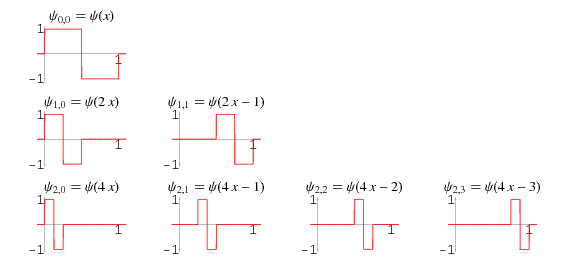
\includegraphics[width=1\textwidth]{./pics/Haar.png}
		\caption{Generation $j=1,2,3$ der Haar-Basis}
		\label{AbbHaarBasis}
	\end{center}
\end{figure}

Jetzt integrieren wir die Wavelets aus Abbildung \ref{AbbHaarBasis} und erhalten die integierte Haar-Basis
\begin{align*}
	H_k(t):=\int\limits_0^t h_k(s)\d s
\end{align*}

%TODO Hier Skizze der integierten Wavelets einfügen (aus den Rechtecken werden Dreiecke)

Approximation der Brownschen Bewegung:\\
\underline{$n=0$}: Man erhält eine zufällige Lineare Funktion.\nl
%TODO Hier Skizze einfügen.
\underline{$n=1$ ($j=0$):}\nl
%TODO Hier Skizze einfügen.
\underline{$n=2$ ($j=2$):}\nl
%TODO Hier Skizze einfügen.
Es kommen also immer neue, zufällige Auslenkungen dazu.\\
\underline{$n$ groß:}
\begin{figure}[H]
	\begin{center}
		%TODO evtl. bessere Skizze erstellen
		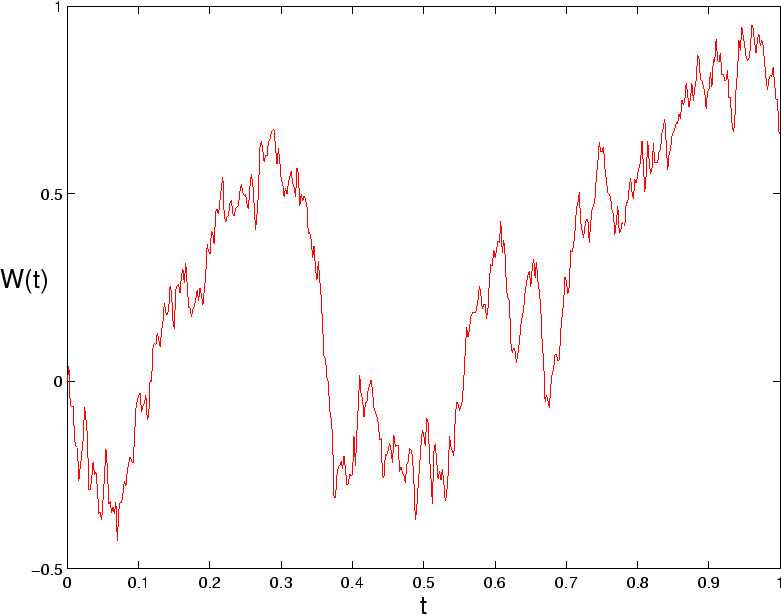
\includegraphics[width=1\textwidth]{./pics/BB.png}
		\caption{Approximation der Brownschen Bewegung für $n$ groß}
		\label{AbbBBngross}
	\end{center}
\end{figure}

\begin{proof}
	Setze
	\begin{align*}
		B_t^N:=\sum\limits_{k=0}^N Z_k\cdot\int\limits_0^t h_k(s)\d s
	\end{align*}
	
	\underline{Zeige a):}
	
	
	\underline{Zeige b):}
	
	\underline{Zeige c:)}
	\begin{align*}
		\E\big[B_t\big]
		&=\E\left[\limn B_t^N\right]
		\overset{a)}=
		\lim\limits_{N\to\infty}\E\left[\sum\limits_{k=0}^N Z_k\cdot H_k(t)\right]
		=\lim\limits_{N\to\infty}\sum\limits_{k=0}^N\underbrace{\E\big[Z_k]}_{=0}\cdot H_k(t)
		=0\\
		\Cov(B_t,B_s)
		&=\E\big[B_t\cdot B_s\big]\\
		&=\E\left[\sum\limits_{k=0}^\infty Z_k\cdot H_k(t)\cdot\sum\limits_{j=0}^\infty Z_j\cdot H_j(s)\right]\\
		&=\sum\limits_{k=0}^\infty\underbrace{\E\big[Z_k\cdot Z_j\big]}_{=\delta_{i,j}}\cdot H_k(t)\cdot H_j(s)\\
		&=\sum\limits_{k=0}^\infty H_k(t)\cdot H_j(s)\\
		&=\sum\limits_{k=0}^\infty \int\limits_0^t h_k(r)\d r\cdot\int\limits_0^s h_k(r)\d r\\
		&=\sum\limits_{k=0}^\infty\left\langle h_k,\indi_{[0,t]}\right\rangle\cdot\left\langle h_k,\indi_{[0,t]}\right\rangle\\
		\overset{\text{Parseval}}&=
		\left\langle\indi_{[0,t]},\indi_{[0,t]}\right\rangle\\
		&=\int\limits_0^{\min\lbrace s,t\rbrace} 1\d r\\
		&=\min\lbrace s,t\rbrace
	\end{align*}
\end{proof}




